\documentclass[11pt,a4paper]{article}

\usepackage[utf8]{inputenc}
\usepackage[T1]{fontenc}
\usepackage{booktabs}
\usepackage{multirow}
\usepackage{array}
\usepackage{graphicx}
\usepackage{amssymb}
\usepackage{amsmath}
\usepackage{textcomp}
\usepackage{float}
\usepackage{url}
\usepackage{hyperref}
\usepackage[capitalize,noabbrev]{cleveref}
\usepackage[margin=1in]{geometry}
\usepackage{threeparttable}
\usepackage[tableposition=top]{caption}
\usepackage{subcaption}
\usepackage{bm}
\usepackage{color}
\usepackage{xcolor}
\usepackage{colortbl}
\usepackage{algorithm}
\usepackage{algorithmic}
\usepackage{times}
\usepackage[numbers]{natbib}

\hypersetup{
  colorlinks=true,
  linkcolor=blue,
  citecolor=blue,
  urlcolor=blue
}

\newcommand{\method}{SharedClass}
\newcommand{\dataset}{SCB5}

\title{Supplementary Material: Shared Class-Neighborhood Geometry: A Candidate Mechanism for Why CLIP Predicts MLLM Difficulty}

\author{
  Lizhuo Zhang\thanks{School of Information and Intelligence, Hunan Agricultural University, Changsha 410128, China. (e-mail: zhanglizhuo@hunau.edu.cn)} \\
  Yan Ma\thanks{School of Foreign Studies, Changsha University of Science and Technology, Changsha 410114, China.}
}

\begin{document}

\renewcommand{\thetable}{S\arabic{table}}
\renewcommand{\thefigure}{S\arabic{figure}}

\maketitle

\section*{Supplementary Perturbation and Prompt-Sensitivity Experiments}
\label{sec:perturb_appendix}

We designed a set of experiments to test \emph{perturbation synchrony}, whether CLIP and MLLM per-class accuracy degrade together under image perturbation, which would directly link shared geometry to shared difficulty. Two attempts are documented below; both remain inconclusive, the first because the target MLLM operates near a performance floor, the second because the perturbation drops of the two model classes are uncorrelated. A complementary \emph{visual-layer} perturbation analysis (same blur pipeline applied to the vision encoders themselves) is reported in Section~4.8 of the main paper and provides supportive, though not decisive, evidence that per-class difficulty changes under blur track each other across independently trained encoders; the MLLM-side attempts remain the primary open gap. We report them here for completeness and to preempt misinterpretation of the results in \path{results/exp_mllm_combined.json}, \path{results/exp4_clip_blur_recreated_all.json}, \path{results/exp_perturbation_blur_dual.json}, \path{results/visual_perturbation_sync_raw.json}, and \path{results/visual_perturbation_sync_raw_all.json}.

\paragraph{MLLM prompt sensitivity is untestable at current accuracy levels.}
On the 8 TeacherBehavior classes (20 images/class), Qwen2-VL-7B scores 15.6\% with bare class-name prompts and an identical 15.6\% with enriched descriptive prompts, yielding no benefit from better prompting. Per-class inspection shows why: the model predicts \texttt{teacher} almost exclusively (19/20 teacher images correct; \texttt{guide} reaches 20\% and all remaining classes at most 5\%), i.e., it has collapsed onto a single class and sits just above the 12.5\% random baseline. Under these floor conditions, the MLLM-side analogue of the prompt experiment of Section~4.5 of the paper (which demonstrated that CLIP's failures are semantic, not visual) cannot run: there is no accuracy headroom in which prompt effects could appear. The same floor defeats blur perturbation on this model: Gaussian blur at $\sigma \in \{0,1,2,4,8\}$ leaves its accuracy approximately flat at 13.1\%, 13.1\%, 12.5\%, 12.5\%, and 11.9\% (at the random baseline throughout), so no degradation gradient is observable.

\paragraph{Blur perturbation under a non-floor MLLM yields no synchrony.}
Because Qwen2-VL-7B operates at the floor, we repeated the blur perturbation with Gemma4-31B (SigLIP ViT-SO400M vision encoder; per-class AnchorScore correlation $\rho=0.725$, among the strongest in our set, Section~4.2), 50 images per TeacherBehavior class ($n=390$), Gaussian blur $\sigma \in \{0,1,2,3,4\}$, scoring responses by display-name match. The baseline escapes the floor (31.3\% at $\sigma=0$ vs.\ 12.5\% random), but the per-class blur-drop profile does not correlate with CLIP's: Spearman $\rho = +0.245$ between CLIP's and Gemma4-31B's per-class accuracy drops (permutation $p=0.564$ over 10{,}000 shuffles, seed 42; scoring by raw-key gives $\rho=-0.567$, $p=0.135$; a 50-images-per-class CLIP subsample gives $\rho \approx 0.14$, n.s.). For reference, CLIP itself under the same blur schedule (\path{exp4_clip_blur_recreated_all.json}) degrades only where it already makes meaningful decisions: \texttt{blackboard-writing} falls from 46.0\% to 2.5\% ($\sigma=8$), while \texttt{teacher} stays flat (83.8\% to 84.1\%) and classes already near zero stay near zero. We read the absence of blur-drop synchrony as a further indication that the MLLM-side behavioral step is dominated by language-side processes, consistent with the confusion-matrix null of Supplement \S2; the floor and the null together leave the MLLM-side geometry$\to$behavior link without direct perturbation evidence, which we flag as the primary open gap in Section~5.5 of the paper.

\section*{Why We Frame the Mechanism as Geometry Rather Than Confusability}
\label{sec:confusion_null}

The main paper measures \emph{class-neighborhood geometry} directly (CKA, Mantel tests on class-centroid similarity matrices) and treats the further step from geometry to behavioral \emph{confusability} as a defined translation rather than a separately measured link (Section~4.3). We tested that link directly on the one SCB5 per-image MLLM dataset available to us: Gemma4-31B (SigLIP ViT-SO400M vision encoder), evaluated on the TeacherBehavior 8-class subset at 50 images per class ($n=390$, the no-blur baseline of the perturbation pilot). For each image we recovered a predicted class from the model's free-text response via the display-name substring rule of \path{experiments/exp_perturbation_blur.py}, built the $8\times8$ confusion matrix, symmetrized its off-diagonal entries over the 28 unordered class pairs, and correlated the result with the SigLIP class-centroid cosine-similarity matrix used in Section~4.3 of the main paper.

\paragraph{The geometry$\to$confusion link is not detectable within this MLLM.}
Accuracy-normalized confusion propensity (which removes per-class accuracy differences) correlates with SigLIP centroid similarity at Spearman $\rho = +0.092$ ($p = 0.641$; permutation $p = 0.735$ over 10{,}000 class-label shuffles of the confusion matrix against fixed similarity, seed 42); raw symmetrized confusion counts give $\rho = +0.263$ ($p = 0.176$). Both are non-significant at $n=28$. Excluding \texttt{teacher} (the dominant LM-attractor that absorbs 47/50 \texttt{answer} images, 30/50 \texttt{blackBoard}, 24/50 \texttt{screen}, 21/50 \texttt{stand}) yields a 7$\times$7 analysis ($n=21$) that remains null: $\rho = +0.044$ ($p = 0.849$) for normalized confusion, $\rho = +0.158$ ($p = 0.494$) for raw counts. The null is not a method artifact: class-name ordering aligns exactly between the confusion and similarity matrices; the SigLIP similarity matrix has adequate variance (range $[0.867, 0.989]$, std $0.035$, not saturated); and a sanity Mantel test between SigLIP and CLIP ViT-L/14 (OpenAI) centroid matrices reproduces the paper's Section~4.3 result exactly ($\rho = 0.955$, within the reported $0.93$--$0.96$), confirming the loading code is correct.

\paragraph{Interpretation and framing consequence.}
The within-MLLM confusion is dominated by language-model priors and text--image alignment choices rather than by pairwise feature-space geometry. This is consistent with Section~4.5 of the main paper, where CLIP's most striking per-class failures (0\%$\rightarrow$100\% under prompt variants) were shown to arise from text--image misalignment rather than from impoverished visual features: both findings indicate that the behavioral step from features to errors is shaped substantially by alignment and language-side biases, not by the class-neighborhood geometry that the vision encoder makes available. We therefore frame the paper's mechanism as \emph{shared class-neighborhood geometry} (the level the experiments actually measure) rather than as \emph{shared class confusability}, which would conflate the geometric claim with an additional behavioral claim that this test fails to support. A cleaner test on a pure vision encoder (CLIP or SigLIP zero-shot, no LM head) would reduce the encoder/language confound but would inherit its own alignment confounds from the text-prompt side; we note this as a candidate follow-up rather than a deferred obligation, since the present null already supports the paper's framing choice. Script: \path{analysis/confusion_vs_geometry.py}; result: \path{results/confusion_vs_geometry.json}.

\section*{Supplementary Counterfactual Mediation Controls}
\label{sec:mediation_controls}

The main paper's mediation analysis (Section~4.4) uses the leave-one-out cross-model mean per-class accuracy as the mediator. This supplement reports the counterfactual controls referenced in that section, which test whether the indirect effect is an artifact of the mediation pipeline rather than of shared per-class difficulty.

\textbf{Protocol.} All controls reuse the identical cluster-bootstrap pipeline of the main analysis: 10{,}000 resamples of the pooled classes (cluster unit), product-of-coefficients indirect effect on rank-$z$ scores per MLLM, mean across models, percentile 95\% CI and one-sided $p$ (fraction of bootstrap means $\leq 0$), bootstrap seed 20260801. Only the mediator construction differs:

\begin{enumerate}
  \item \emph{Baseline} (replication): $M_j$ = mean per-class accuracy of the eight other MLLMs (leave-one-out), as in the main paper. The SCB5 result must reproduce the combined-test numbers reported in Section~4.4.
  \item \emph{Class-permuted}: the baseline mediator with class labels permuted by a single fixed permutation (seed 42), preserving its marginal rank structure while destroying per-class signal.
  \item \emph{Random noise}: one fixed per-model uniform noise vector (seeded), carrying no difficulty information.
  \item \emph{Independent encoder} (SCB5 only): per-class accuracy of OpenAI ViT-L/14 and ViT-B/32 on the same evaluation pipeline and image set as AnchorScore but with checkpoints outside both the LAION-2B anchor and the nine-model MLLM set, taken from the committed multi-backbone snapshot. Stanford40 has no multi-backbone anchors, so this control cannot run there.
\end{enumerate}

\textbf{Results.} Table~\ref{tab:mediation_controls} reports the cross-model mean indirect effect under each mediator specification.

\begin{table}[H]
\centering
\caption{Cross-model mean indirect effect under the counterfactual mediator specifications. Point: full-data cross-model mean of per-model indirect effects (the convention of the main-paper combined test); CI: 95\% percentile interval over bootstrap means; $p$: one-sided.}
\label{tab:mediation_controls}
\small
\begin{tabular}{lcccc}
\toprule
Mediator specification & Point & 95\% CI & $p$ (one-sided) & Excl.\ 0 \\
\midrule
\multicolumn{5}{c}{\textit{SCB5 ($n=13$ classes, 9 MLLMs)}} \\
\midrule
Baseline LOO mean (replication) & $+0.536$ & [$-$0.515, $+0.888$] & 0.089 & no \\
Class-permuted LOO mean & $-$0.042 & [$-$0.319, $+0.106$] & 0.741 & no \\
Random noise & $-$0.018 & [$-$0.141, $+0.068$] & 0.758 & no \\
OpenAI ViT-L/14 (independent encoder) & $+0.005$ & [$-$0.213, $+0.390$] & 0.416 & no \\
OpenAI ViT-B/32 (independent encoder) & $+0.003$ & [$-$0.132, $+0.152$] & 0.465 & no \\
\midrule
\multicolumn{5}{c}{\textit{Stanford40 ($n=40$ classes, 6 MLLMs)}} \\
\midrule
Baseline LOO mean & $+0.562$ & [$+0.371$, $+0.708$] & $<0.0001$ & \textbf{yes} \\
Class-permuted LOO mean & $-$0.006 & [$-$0.055, $+0.042$] & 0.620 & no \\
Random noise & $-$0.018 & [$-$0.058, $+0.017$] & 0.835 & no \\
\bottomrule
\end{tabular}
\end{table}

\textbf{Interpretation.} On Stanford40, where the analysis is powered, the baseline indirect effect is positive and excludes zero while both counterfactual mediators produce indirect effects statistically indistinguishable from zero and negative in sign: the pipeline attributes nothing when the mediator's per-class signal is destroyed, and the significant baseline result is specific to the genuine shared-difficulty mediator. On SCB5 the baseline reproduces the main-paper combined test exactly (point $+0.536$ vs.\ reported $+0.54$; CI $[-0.515, +0.888]$ vs.\ $[-0.51, +0.89]$; $p=0.089$), and the permuted and noise mediators again collapse. The independent-encoder controls are not significant on SCB5, but their $a$-path to the anchor is much weaker than that of the LOO MLLM mean (Spearman $\rho = 0.236$--$0.599$ vs.\ $0.874$; approximate VIF 1.1--1.6 vs.\ 4.2), so at $n=13$ these controls are uninformative either way; Stanford40, which has the power, cannot run them. The three controls together establish that the mediation result is not a pipeline artifact and is specific to a mediator that carries shared per-class difficulty information.

\section*{Supplementary Per-Model Correlation Table}
\label{sec:per_model_table}

Table~\ref{tab:per_model_rho} reports the per-model AnchorScore--MLLM Spearman correlations summarized in Section~4.1 of the main paper, grouped by vision-encoder family as in Section~4.2. The six Qwen3.x and Gemma4 models use the frozen per-class accuracies of the AnchorScore benchmark \cite{la}; the three LLaVA models (LLaVA-1.5-13B, LLaVA-NeXT-Mistral-7B, LLaVA-NeXT-Vicuna-7B) are evaluated in this work with the identical protocol (class-name prompt, 100 images per class, fixed seed; \path{experiments/eval_hf.py}). LLaVA-1.5-7B follows the original benchmark evaluation. Group means: CLIP $0.462$, SigLIP $0.716$, QwenViT $0.669$ (\path{analysis/kruskal_4groups.py}, output \path{results/kruskal_4groups.json}).

\begin{table}[H]
\centering
\caption{Per-model AnchorScore--MLLM per-class Spearman correlations on SCB5 ($n=13$ classes), grouped by vision-encoder family. $p$: two-sided Spearman.}
\label{tab:per_model_rho}
\small
\begin{tabular}{llcc}
\toprule
Model & Encoder family & $\rho$ & $p$ \\
\midrule
\multicolumn{4}{c}{\textit{CLIP group}} \\
\midrule
LLaVA-NeXT-Mistral-7B & CLIP & 0.521 & 0.068 \\
LLaVA-1.5-7B & CLIP & 0.473 & 0.103 \\
LLaVA-1.5-13B & CLIP & 0.454 & 0.119 \\
LLaVA-NeXT-Vicuna-7B & CLIP & 0.402 & 0.173 \\
\midrule
\multicolumn{4}{c}{\textit{SigLIP group}} \\
\midrule
Gemma-3-27B & SigLIP & 0.687 & 0.010 \\
Gemma4-31B & SigLIP & 0.725 & 0.005 \\
Gemma4-26B-A4B & SigLIP & 0.736 & 0.004 \\
\midrule
\multicolumn{4}{c}{\textit{QwenViT group}} \\
\midrule
Qwen3.5-35B-A3B & QwenViT & 0.736 & 0.004 \\
Qwen3.6-35B-A3B & QwenViT & 0.687 & 0.010 \\
Qwen3.6-27B & QwenViT & 0.648 & 0.017 \\
Qwen3.5-27B & QwenViT & 0.604 & 0.029 \\
\midrule
\multicolumn{4}{c}{\textit{Qwen2-VL ViT group}} \\
\midrule
Qwen2-VL-7B & Qwen2-VL ViT & 0.374 & 0.209 \\
\bottomrule
\end{tabular}
\end{table}

\section*{Supplementary CKA Matrix}
\label{sec:cka_matrix}

The full matrix is shown in \Cref{fig:cka_matrix}.

\begin{figure}[H]
\centering
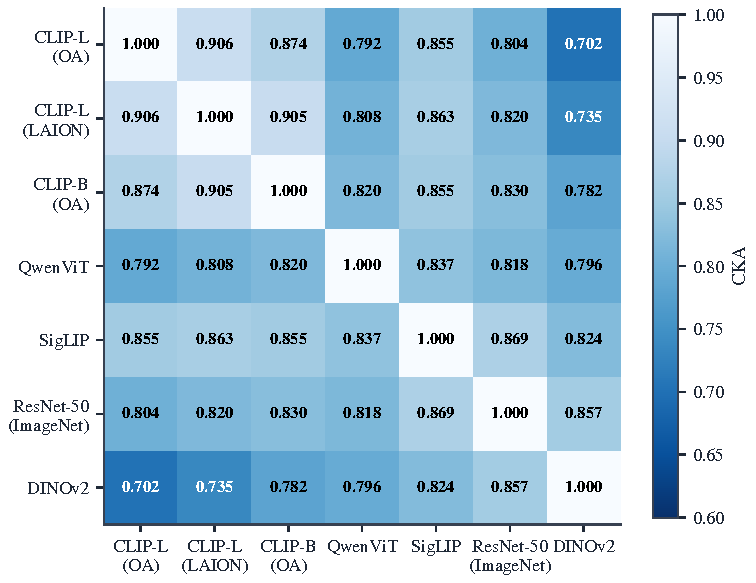
\includegraphics[width=0.8\textwidth]{figures/figS1_cka_heatmap.pdf}
\caption{Pairwise linear CKA between the seven vision encoders used in Section~4.3 of the main paper (computation described in the same section). Features are extracted from 160 SCB5 images (20 per class, TeacherBehavior) and L2-normalized before CKA. The matrix supports the values cited inline in Section~4.3: within-CLIP CKA $\geq 0.87$; cross-Internet-scale CKA (CLIP vs.\ QwenViT, CLIP vs.\ SigLIP) $0.79$--$0.86$; the two more constrained controls reach $0.80$--$0.87$ (ResNet-50, ImageNet-1k only) and $0.70$--$0.82$ (DINOv2, LVD-142M) against the Internet-scale encoders, with DINOv2 the only encoder pair dropping to $0.70$. Color scale $[0.6, 1.0]$.}
\label{fig:cka_matrix}
\end{figure}

\bibliographystyle{elsarticle-num}
\bibliography{refs}

\end{document}